\specialsection{Обзор литературы}

Тема применения нейронных сетей в контексте решения формально-логических задач развита не особо сильно, поскольку дискретные задачи со строгими ограничениями тяжело даются сетям с известными на данный момент архитектурами. Тем не менее, известны многочисленные попытки использовать нейросети в качестве помощника для алгоритма, решающего ту или иную задачу. Несколько таких подходов, имеющих отношение к проверке выполнимости и поиску решения для SMT-формул, я рассмотрю далее.

\specialsubsection{FastSMT}

В статье \cite{fastsmt-paper} рассматривается идея повышения эффективности SMT-решателя за счёт оптимизации его работы на формулах, возникающих в задачах из фиксированной предметной области.

Решатель в процессе своей работы применяет к формуле большое количество разных семантически эквивалентных преобразований\footnote{В статьях и документациях их называют тактиками.}, чтобы привести её к некоторому удобному для себя виду, в котором он сможет либо достаточно быстро найти решение для формулы и доказать, что оно подходит (тем самым доказав, что формула является выполнимой), либо достаточно быстро доказать, что указанный в формуле набор ограничений невозможно выполнить, и формула является невыполнимой. Примеры тактик: замена переменной, нормализация границ неравенства, bit-blasting (представление переменной в виде набора пропозициональных значений), переписывание условного оператора через конъюнкцию импликаций и т. д.. Упомянутый ранее решатель Z3 \cite{z3-paper} поддерживает более ста подобных операций.

Цепочка преобразований, которые решатель производит над формулой, формируется согласно некоторой стратегии, которая учитывает самые разнообразные параметры\footnote{Будем также называть их признаками.} формулы: от её размера и количества свободных переменных до некоторого приближения абстрактно-синтаксического дерева формулы. Сама стратегия, в данном случае, больше всего похожа на решающее дерево, у которого в вершинах стоят ограничения на очередные параметры формулы, а в каждом листе находится тактика, которую стоит применить в случае, когда параметры соответствуют пути в этот лист.

Базовую стратегию, которая используется в решателе по-умолчанию, подбирают его создатели, причём они делают это так, чтобы его средняя скорость работы на произвольной формуле была как можно лучше. В результате, решатель работает более стабильно (т. е. реже уходит в экспоненциальный перебор возможных решений, когда на вход подают сложную формулу), но скорость нахождения ответа в более простых случаях из-за этого проседает.

В то же время, большинство популярных современных инструментов для решения SMT-формул поддерживают возможность использования специфических стратегий, которые можно построить, в том числе, самостоятельно. Помимо этого, есть некоторая интуиция, что если мы будем рассматривать только формулы из некоторой фиксированной практической задачи, то все эти формулы будут обладать некоторой спецификой, знание о которой сможет существенно помочь в проверке их выполнимости. На этой интуиции, а также на возможности использовать собственные стратегии при решении формул строится подход, описанный в рассматриваемой статье.

Главная идея состоит в следующем: набор признаков формулы можно рассматривать как состояние некоторой среды, применение очередной тактики можно рассматривать как некоторое действие, совершаемое в этой среде, а награду за последовательность применённых тактик можно определить как суммарное время работы решателя на заданной формуле с использованием этой последовательности (разумеется, взятое с минусом), либо какому-нибудь штрафному значению в случае, если решатель не справляется с формулой. Таким образом, задача поиска оптимальной стратегии применения различных тактик хорошо представляется в виде задачи обучения с подкреплением, где средой является произвольная формула из некоторой фиксированной задачи. Поэтому предлагается выучивать модель (политику), которая по текущему состоянию среды (формулы) будет выдавать оптимальную тактику и параметры для неё.

\begin{figure}[ht]
\begin{center}
    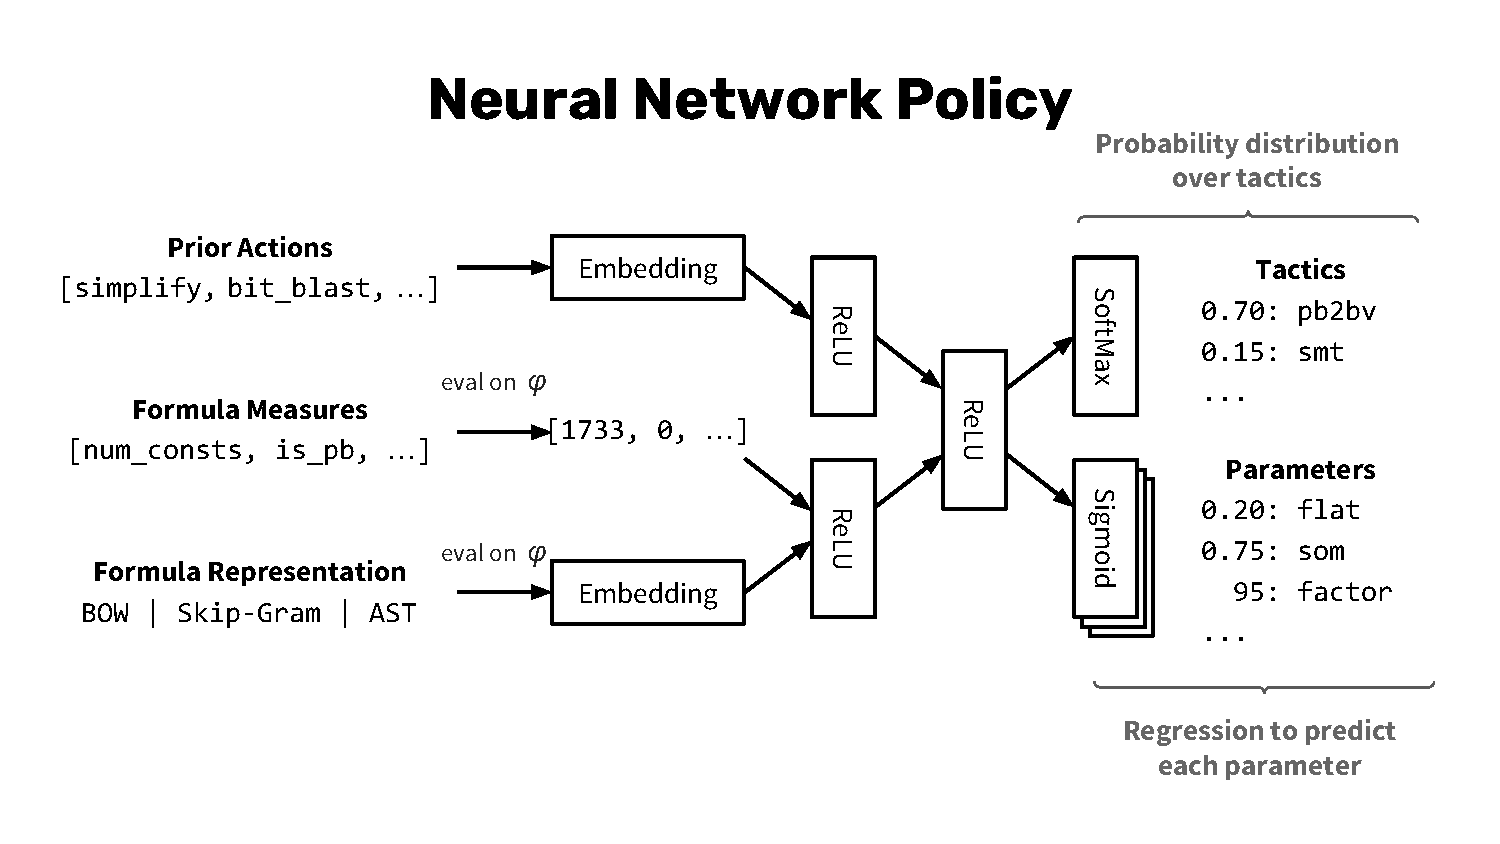
\includegraphics[scale=0.65]{./assets/fastsmt-nn-policy.pdf}
    \caption{\label{fastsmt-architecture} Архитектура модели. Картинка взята из статьи \cite{fastsmt-paper}.}
\end{center}
\end{figure}

Архитектура модели изображена на рис.~\ref{fastsmt-architecture}. На вход подаются признаки формулы (Formula Measures) и её синтаксическое представление, закодированное в виде bag-of-words или $n$-граммной модели (Formula Representation). Вдобавок к этому, для каждой тактики выучивается эмбеддинг\footnote{От англ. \textit{embedding} --- в машинном обучении так называют представление некоторого объекта в многомерном векторном пространстве.}, который хранит в себе семантическую информацию про неё. Эмбеддинги тактик, которые можно применить в данный момент, также подаются на вход модели (Prior Actions). На выходе у модели распределение на тактиках, которые стоит применить в данный момент, и значения параметров для них. Сразу отмечу, что, несмотря на то, что модель выдаёт распределение на всех доступных для применения в данный момент тактиках, за одно действие применяется только одна из них --- наиболее вероятная.

Построенная таким образом модель обучается на наборе формул взятом из некоторой задачи (в статье это были различные известные бенчмарки для решателей, на каждом из которых обучалась и оценивалась отдельная модель) с помощью метода, похожего на кросс-энтропийный метод. После этого с помощью техник семплирования строятся разнообразные статистики, отражающие выученную моделью политику, а уже на них обучается решающее дерево, выбирающее нужную тактику по текущей формуле, которое впоследствии превращается в стратегию, которую можно загрузить в SMT-решатель.

Авторы статьи заявляют, что, согласно проведённым экспериментам, предложенный подход позволяет успешно решать на 17\% больше формул при десятисекундном ограничении по времени, а также даёт прирост производительности вплоть до стократного ускорения на некоторых формулах (при этом, замедления при решении других формул не наблюдается). Тем не менее, у такого подхода есть существенный недостаток: для каждой новой задачи нужно сначала самостоятельно собирать данные, потом запускать тяжеловесный процесс обучения, а после этого самому синтезировать стратегию. Это требует довольно больших вычислительных мощностей.

\specialsubsection{GNN for Scheduling of SMT Solvers}

В статье \cite{gnn-for-scheduling-paper} рассматривается более общий подход к задаче: известно, что в основе работы разных SMT-решателей лежат разные алгоритмы и эвристики, поэтому их производительность при решении разных формул может значительно варьироваться; в связи с этим, давайте просто обучим модель, которая по формуле будет предсказывать, за какое время тот или иной решатель сможет проверить её на выполнимость, а далее перед каждой проверкой будем выбирать решатель, для которого модель предсказывает наименьшее время работы.

Данная статья интересна тем, что в ней рассматривается более точное представление формулы, подаваемой модели на вход. Вместо сбора разных статистик с формулы и превращения их в признаки авторы предлагают использовать графовую нейронную сеть\footnote{Далее по тексту будем называть их GNN (англ. \textit{Graph Neural Networks}).}, которая задействует абстрактно-синтаксическое дерево\footnote{Далее в тексте будет использоваться аббревиатура AST (англ. \textit{Abstract-Syntax Tree}).} формулы в качестве графа вычислений (рис.~\ref{gnn-for-scheduling-architecture}).

\begin{figure}[ht]
\begin{center}
    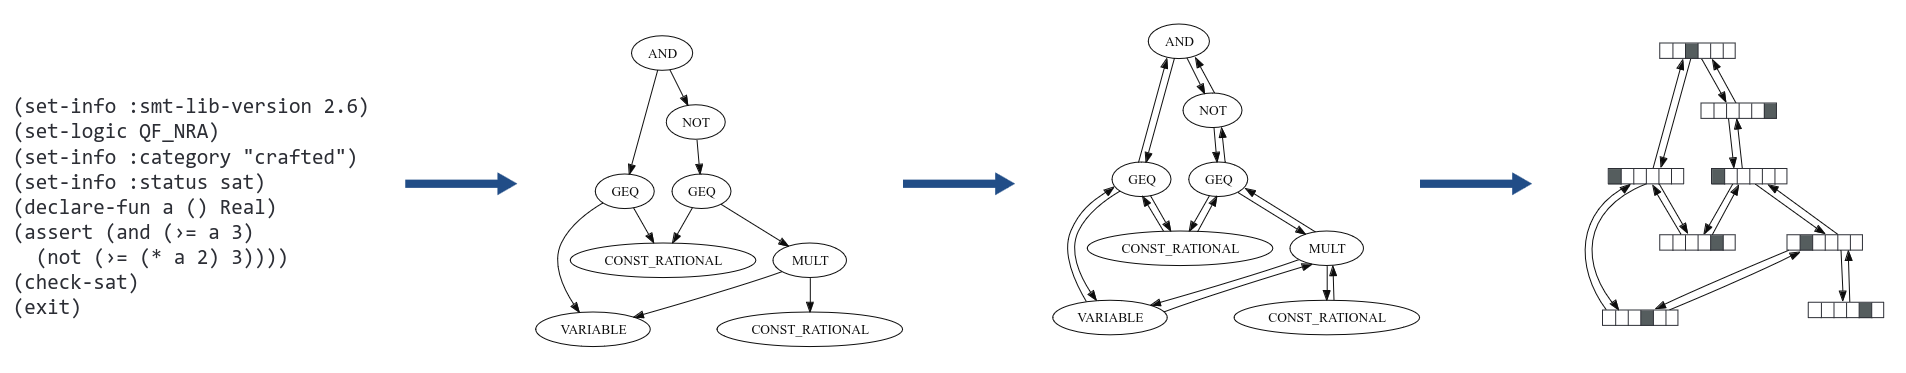
\includegraphics[scale=0.24]{./assets/gnn-for-scheduling-architecture.png}
    \caption{\label{gnn-for-scheduling-architecture} Использование AST формулы в качестве графа вычислений для GNN. Картинка взята из статьи \cite{gnn-for-scheduling-paper}.}
\end{center}
\end{figure}

Чтобы ускорить работу, вершины дерева, отвечающие за эквивалентные выражения, склеиваются в одну, так что формула, на самом деле, превращается в ориентированный ациклический граф. Помимо этого, чтобы расширить распространение эмбеддинга с информацией, сохранённой в каждой вершине, к каждому ребру такого графа добавляется обратное ребро. Таким образом, информация начинает распространяться сразу во всех направлениях.

Далее каждая вершина (переменная, константа или операция) кодируется с помощью техники one-hot-encoding, после чего векторы с полученными таким образом значениями отправляются в GNN\footnote{Более подробно про работу графовых нейронных сетей будет написано далее в соответствующей главе.}, на выходе у которой находится слой, собирающий эмбеддинги со всех вершин графа и предсказывающий для каждого SMT-решателя время, за которое он может выдать ответ на данной формуле. Для лучшего понимания, схема процесса изображена на рис~\ref{gnn-for-scheduling-process}.

\begin{figure}[ht]
\begin{center}
    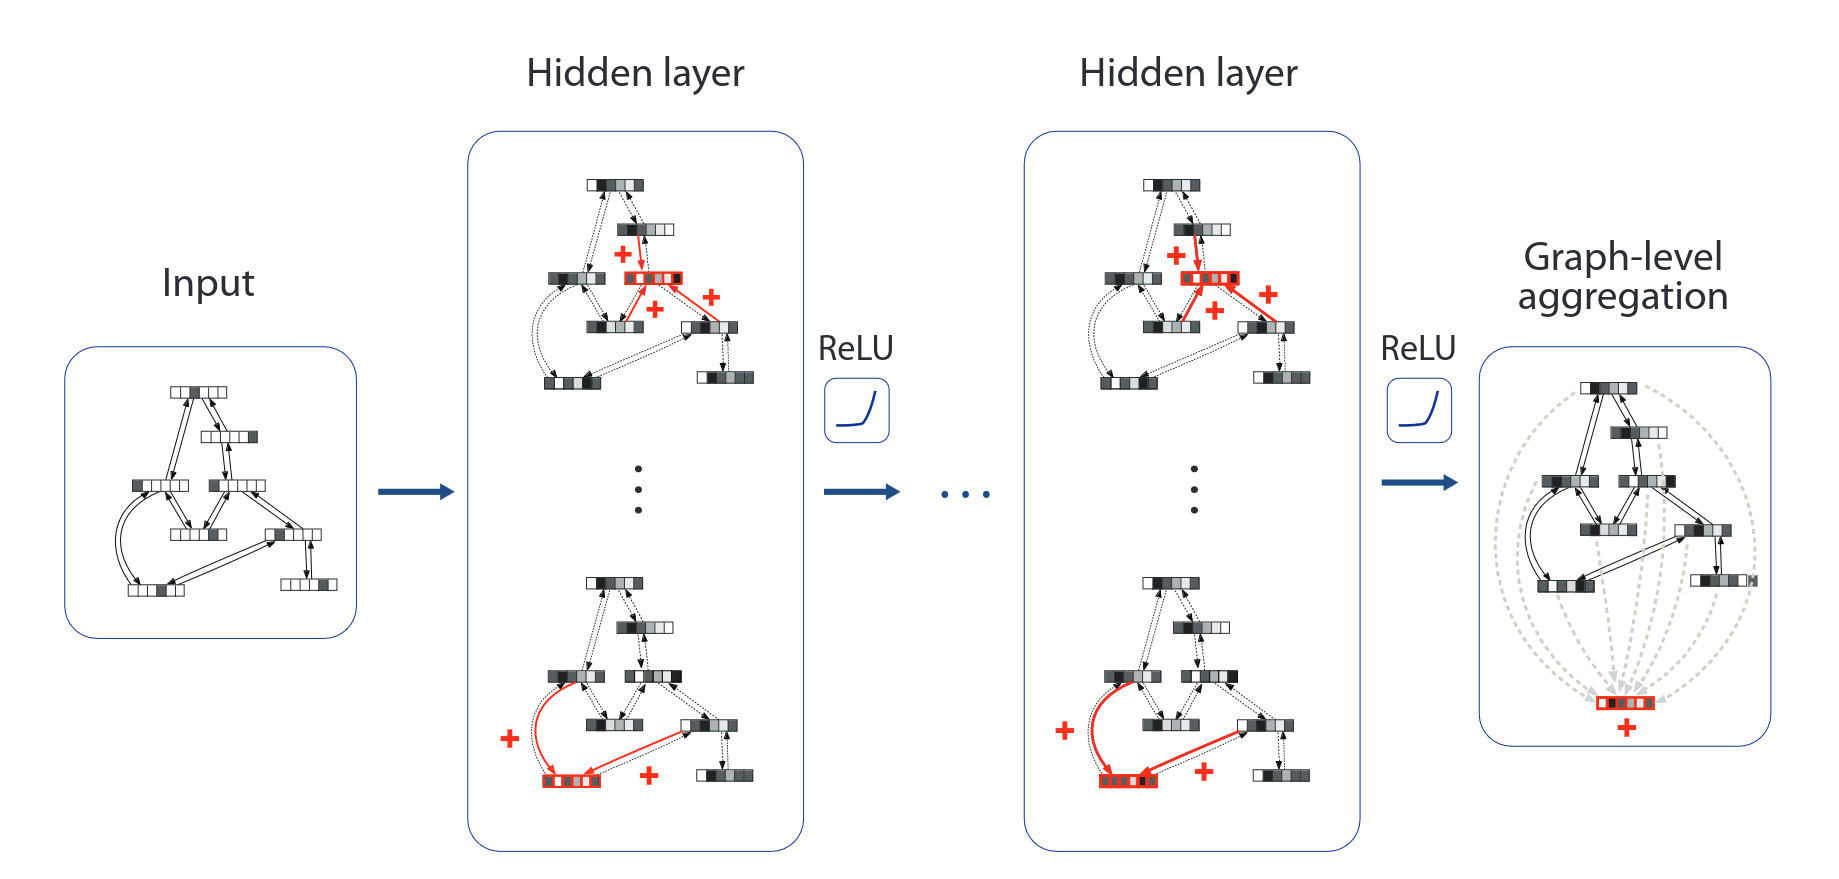
\includegraphics[scale=0.25]{./assets/gnn-for-scheduling-process.png}
    \caption{\label{gnn-for-scheduling-process} Схема использования GNN для получения информации о формуле и предсказания ответа. Картинка взята из статьи \cite{gnn-for-scheduling-paper}.}
\end{center}
\end{figure}

Авторы отмечают, что подход может быть применён для решения почти для любой SMT-формулы, и утверждают, что им удалось добиться ускорения процесса на 8--900\% на разных тестах.

\specialsubsection{NeuroSAT}

Тем не менее, попытки научиться решать формально-логическую задачу, пользуясь исключительно нейронными сетями, тоже присутствуют. Пионером в этой области стала работа \cite{neurosat-paper}, в которой исследовалось применение GNN для задачи SAT. Была предложена следующая графовая архитектура: для каждой переменной, для отрицания каждой переменной и для каждого конъюнкта формулы заводится по вершине; далее рёбра проводятся между парами из литерала (переменными или их отрицаниями) и конъюнкта, если литерал входит в состав конъюнкта, а также между парами противоположных литералов (теми, которые является отрицаниями друг друга). Пример построения такого графа изображён на рис.~\ref{neurosat-mpnn}.

\begin{figure}[ht]
\begin{center}
    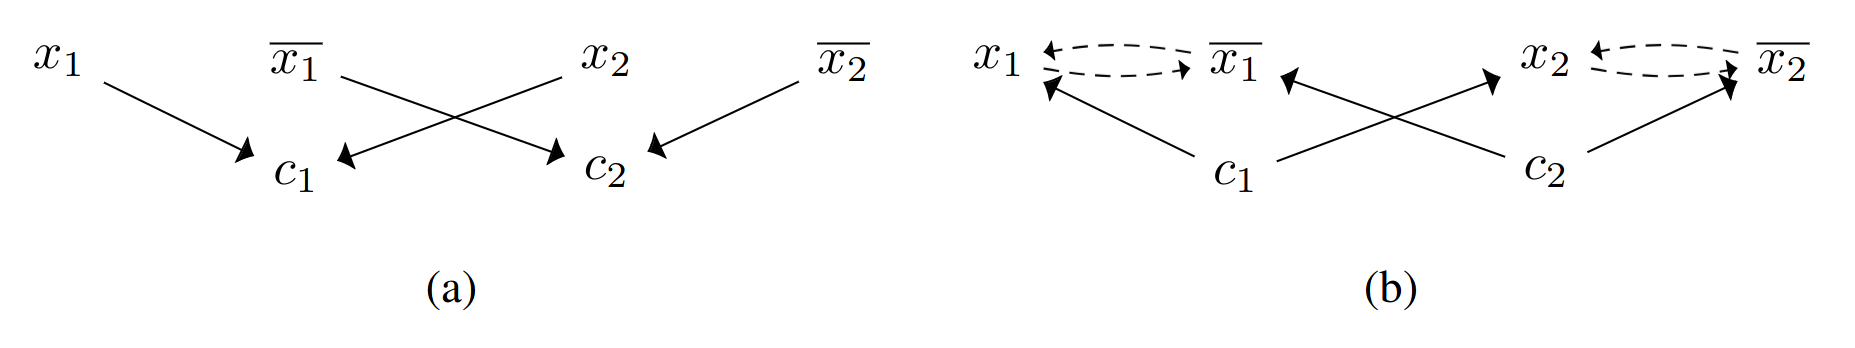
\includegraphics[scale=0.25]{./assets/neurosat-mpnn.png}
    \caption{\label{neurosat-mpnn} Граф, построенный для формулы $(x_1 \vee x_2) \wedge (\overline{x_1} \vee \overline{x_2})$. Пункты (a) и (b) отражают шаги построения, описанные в статье; на деле же граф выглядит как их объединение. Картинка взята из статьи \cite{neurosat-paper}.}
\end{center}
\end{figure}

Во время вычислений каждая вершина накапливает все пришедшие к ней сообщения с помощью LSTM\footnote{Долгая краткосрочная память (от англ. \textit{Long Short-Term Memory} --- известная модификация рекуррентной нейронной сети}-слоя. После очередного шага передачи сообщений по графу каждая вершина-литерал генерирует собственное предсказание по поводу того, является ли данная формула выполнимой (внутреннее состояние LSTM отправляется в MLP\footnote{Многослойный перцептрон (от англ. \textit{Multi-Layer Perceptron}) --- последовательная комбинация из полносвязных линейных слоёв и нелинейных слоёв активации.}, который предсказывает одно число --- степень уверенности вершины в том, что формула выполнима).

\begin{figure}[ht]
\begin{center}
    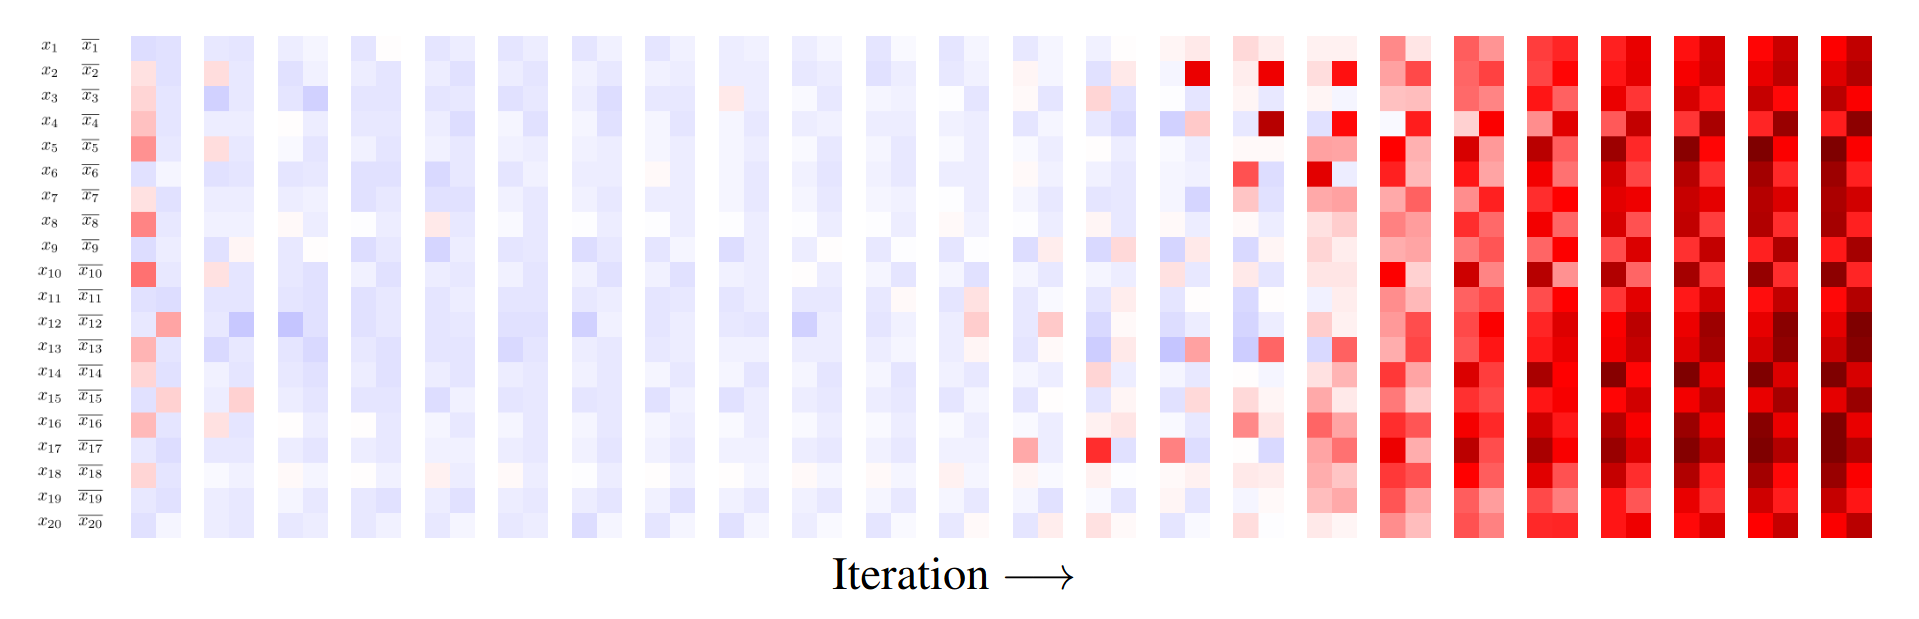
\includegraphics[scale=0.24]{./assets/neurosat-voting.png}
    \caption{\label{neurosat-voting} Граф, построенный для формулы $(x_1 \vee x_2) \wedge (\overline{x_1} \vee \overline{x_2})$. Пункты (a) и (b) отражают шаги построения, описанные в статье; на деле же граф выглядит как их объединение. Картинка взята из статьи \cite{neurosat-paper}.}
\end{center}
\end{figure}

% эмбеддинги
% слой голосования
% итерации
% результаты
% случайные формулы

% \hrule

% todo: дописать про другие работы
% \specialsubsection{Другие работы}

% mach smt
% alpha geometry
% https://ruoyuwang.me/bar2019/pdfs/bar2019-final80.pdf
% https://www.semanticscholar.org/paper/Algorithm-selection-for-SMT-Scott-Niemetz/aff1afe03f8e2f636b972add9b03ac59f6c34223
% https://www.semanticscholar.org/paper/On-EDA-Driven-Learning-for-SAT-Solving-Li-Shi/5c4bb681fe5cb159b0d577b784fa52c952871e17
% https://www.semanticscholar.org/paper/SATformer%3A-Transformer-Based-UNSAT-Core-Learning-Shi-Li/06547a615390ba14d37c684136c30a4ac559d610
% https://www.semanticscholar.org/paper/NeuroBack%3A-Improving-CDCL-SAT-Solving-using-Graph-Wang-Hu/a613142147ef740b2daf1265e23606c80d1c2bd2
% https://www.semanticscholar.org/paper/Synthesizing-Smart-Solving-Strategy-for-Symbolic-Chen-Chen/c7f8cd87ae269bb8b85eeb627005b7884a81bee0
